\RequirePackage{ifluatex}
\ifluatex
  \RequirePackage{pdftexcmds}
  \makeatletter
  \let\pdfstrcmp\pdf@strcmp
  \let\pdffilemoddate\pdf@filemoddate
  \makeatother
\fi

\documentclass[25pt, a0paper, landscape, fleqn]{tikzposter}

% \usepackage[colalign]{myposter}

% \tikzposterlatexaffectionproofoff

%% load packages

\usepackage{blindtext, comment, setspace}

\usepackage{geometry}

\usepackage{tikz, pgfplots, xcolor}

\pgfplotsset{compat=1.16}

\usepackage{amsmath, amssymb, mathtools}

\usetikzlibrary{arrows.meta, calc}

\usepackage[siunitx]{circuitikzgit}

\usepackage[backend=biber, style=authortitle-terse]{biblatex}
\addbibresource{References.bib}



\tikzset{
neuron/.style={
  % The shape:
  circle,
  % The size:
  minimum size=6mm,
  % The border:
  very thick,
  draw=blue!50!black!50,
      % The filling:
  top color=white,
  bottom color=blue!50!black!20, % and something else at the bottom
  % Font
  font=\itshape,
  % padding around node
  outer sep=2mm
  }
}

\newcommand{\dd}[2]{% double diffusion arrows
  \draw  [-Circle] ($(#1.north east)!0.7!(#1.north)$) -- ($(#2.south east)!0.7!(#2.south)$);
  \draw  [Circle-] ($(#1.north west)!0.7!(#1.north)$) -- ($(#2.south west)!0.7!(#2.south)$);
  }

\newcommand{\sd}[2]{% single diffusion arrows
  \draw [-Latex] (#1.east) -- (#2.west);
  }

\usepgfplotslibrary{colormaps, colorbrewer}

\pgfplotsset{compat=1.16}

\usepackage{listings}

\lstset{
  stepnumber=2,
  numbersep=5pt,
  language = python,
  basicstyle=\tiny,
  keywordstyle = \color{blue}\bfseries,
  emph = {FHND, odeint},
  emphstyle = \color{brown}\bfseries,
  commentstyle=\color{gray}\itshape,
}

% \tikzexternalize

%% setup document

% \geometry{paperheight=46.8in, paperwidth=37in, landscape}

% \settitle{ \centering \hbox{\@titlegraphic  \vbox{
%      \centering
%     \color{titlefgcolor} {\bfseries \Huge \@title \par}
%     \vspace*{1em}
%     {\huge \@author \par} \vspace*{1em} {\LARGE \@institute}}
% }}
\makeatletter
\renewcommand\TP@maketitle{%
   \begin{minipage}{44.6in}
        \centering
        \color{titlefgcolor}
        {\bfseries \Huge \@title \par}
        \vspace*{1em}
        {\huge \@author \par}
        \vspace*{1em}
        {\LARGE \@institute}
    \end{minipage}%
    % \hfill
    \begin{minipage}{2in}
       \centering
       \hspace{-6in}
       \@titlegraphic
    \end{minipage}
}
\makeatother

\title{A biomimetic reaction diffusion network simulates C. elegans motion}
\author{Anshul Singhvi, Rifah Tasnim}
\date{\today}
\institute{Bard College at Simon's Rock}
\titlegraphic{
            % \hspace{3in}
            
\includegraphics[height=2in]{sr-pdf-white}
            % \hspace{-10in}
            }
\usetheme{Autumn}
\usecolorstyle{Denmark}
\defineblockstyle{Slide}{
    titlewidthscale=1, bodywidthscale=1, titleleft,
    titleoffsetx=0pt, titleoffsety=0pt, bodyoffsetx=0pt, bodyoffsety=0pt,
    bodyverticalshift=0pt, roundedcorners=0, linewidth=0pt, titleinnersep=1cm,
    bodyinnersep=1cm
}{
    \ifBlockHasTitle%
        % changed "right color=..,left color=.." to "fill=blocktitlebgcolor"
        \draw[draw=none, fill=lightgray]
           (blocktitle.south west) rectangle (blocktitle.north east);
    \fi%
    \draw[draw=none, fill=blockbodybgcolor] %
        (blockbody.north west) [rounded corners=30] -- (blockbody.south west) --
        (blockbody.south east) [rounded corners=0]-- (blockbody.north east) -- cycle;
}

\begin{document}

\maketitle

\onehalfspacing
% \large

\begin{columns}


  \column{0.33333333}

  \block{Abstract}{
    The nematode \textit{Caenorhabditis elegans} is a popular model organism, with a very simple, well-⁠mapped neuronal structure (302 neurons). It moves using undulatory, quasi-⁠sinusoidal motion, apparently generated by a simple central pattern generator (CPG). We aimed to simulate the dynamics of its CPG with a network of the simplest biomimetic model neurons, FitzHugh-⁠Nagumo (FHN) neurons, using the SciPy ODE solver.  The FHN model consists of two differential equations -⁠ membrane potential and a slow inhibitor.  Gap junctions and inhibitory synapses were modeled with one-⁠way diffusion, the latter with a negative diffusion constant.  The network drove a simulated muscle structure which generated undulations resembling \textit{C. elegans}. We also developed a prototype analog electronic implementation based on Keener's circuit, mimicking FHN dynamics, and found coupling mechanisms which reproduced key features of \textit{C. elegans} dynamics. The next goal is to simulate \textit{C. elegans} undulation with analog circuits.  This work was performed at the Hastings lab (Simon’s Rock), collaborating with Jenny Magnes’ VAOL lab (Vassar).
  }

  \block{The math}{
  The FitzHigh-Nagumo equations have the form:
  \[
  \begin{aligned}
    &\frac{d v}{d t}=v-\frac{v^{3}}{3}-w+I\\
    &\frac{d w}{d t}=\epsilon(v-\gamma w+\beta)
  \end{aligned}
  \]
  where $v$ is the membrane potential, and $w$ is a slow inhibitor variable.  D can be positive (excitatory synapses, gap junctions) or negative (inhibitory junctions).

  Implementation of diffusion coupling leads to the addition of a term $D\cdot \mathrm{max}\left(\Delta V,\ 0\right)$ to the membrane potential.
  }

  \block{The worm}{
  \textit{Caenorhabditis elegans} is a small nematode with a well-known neuronal layout.  Its central pattern generator can be sufficiently approximated by a network of only six neurons, arranged as such:
  % \begin{minipage}{\pagewidth}
    % \begin{tikzfigure}[Central pattern generator schematics]
    %   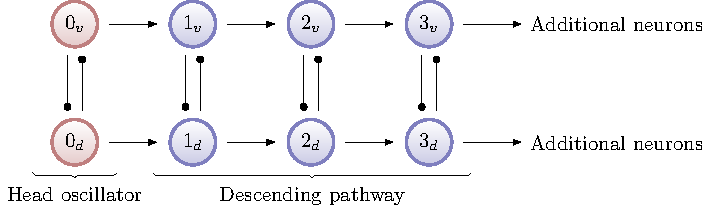
\includegraphics[width = 0.125\pagewidth]{./Figures/CPG/CPG.pdf}
    % \end{tikzfigure}
  % \end{minipage}

  \begin{minipage}[b]{0.15\pagewidth}
    \begin{tikzfigure}[Central pattern generator simplified]
      \centering
      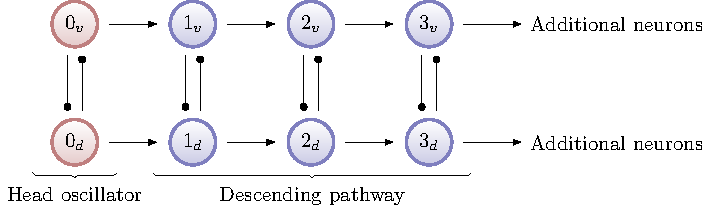
\includegraphics[width = 0.125\pagewidth]{./Figures/CPG/CPG.pdf}
    \end{tikzfigure}
  \end{minipage}
  \begin{minipage}[b]{0.15\pagewidth}
    \begin{tikzfigure}[CPG from Xu \textit{et al}]
      \centering
      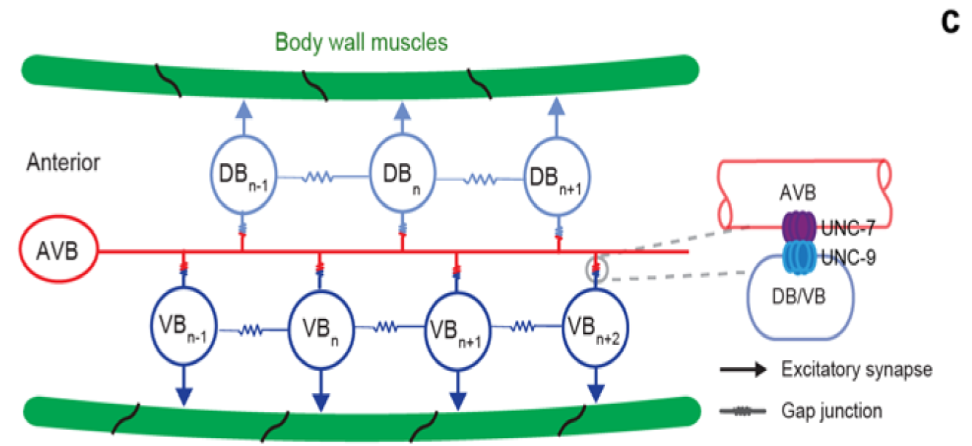
\includegraphics{./Figures/xu_cpg.png}
    \end{tikzfigure}
  \end{minipage}

  wherein 
\includegraphics[height = 0.65\baselineskip]{./Figures/2sh/2sh.pdf} represents unidirectional diffusion coupling, and 
\includegraphics[height = 0.65\baselineskip]{./Figures/2dh/2dh.pdf} represents bidirectional diffusion coupling.
  }

  \column{0.33333333}

  \block{Simulations}{
  We solved these differential equations with different parameter sets using SciPy's ODE solver.

  \vspace{0.8\baselineskip}

  \begin{tikzfigure}[Responses to coupling]
    \centering
    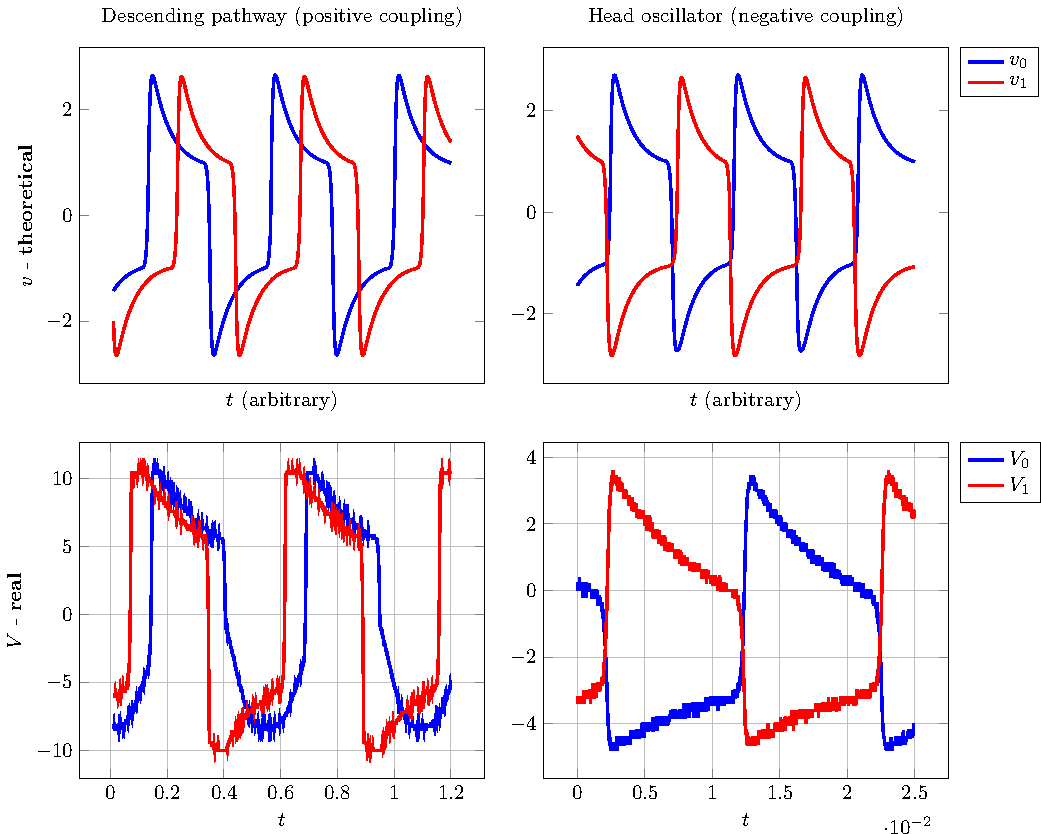
\includegraphics[width=0.29\pagewidth]{./Figures/ReallyTheoretical/ReallyTheoretical.pdf}
  \end{tikzfigure}

  \vspace{\baselineskip}

  \begin{tikzfigure}[Simulated worm motion]
    \centering
    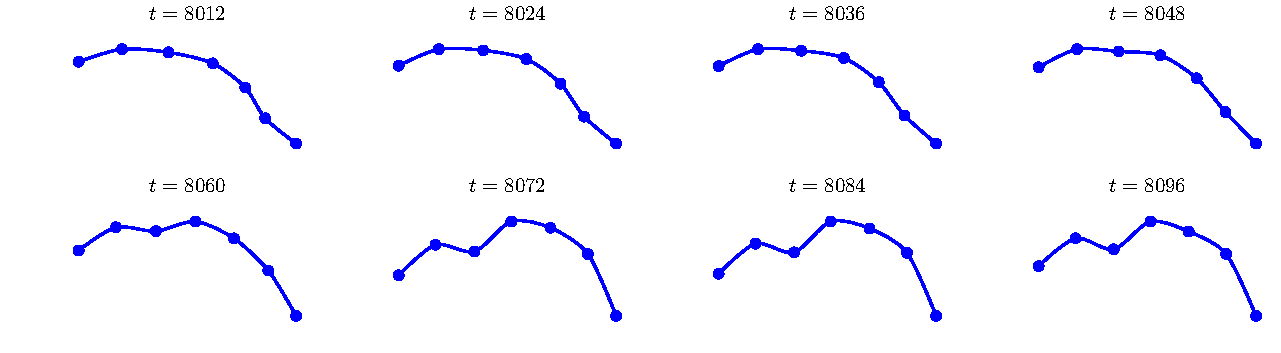
\includegraphics[width=0.3\pagewidth]{./Figures/Worms/Worms.pdf}
  \end{tikzfigure}
  }

  \block{Minimal code example}{
  \begin{minipage}[b]{0.15\pagewidth}
    \lstinputlisting[frame = tRb, lastline = 14]{minimalode.py}
  \end{minipage}
  \begin{minipage}[b]{0.15\pagewidth}
    \lstinputlisting[frame = tbL, firstline = 15]{minimalode.py}
  \end{minipage}
  }

  \column{0.33333332}

  \block{The circuit}{

  The FitzHugh-Nagumo equations translate directly into a circuit that uses inductors, as $L = \frac{dI}{dt}$; however, that is an expensive and impractical solution due to mutual inductance effects.  Keener's circuit proposes a simulation of the inductors with operational amplifiers, which make the circuit considerably cheaper, stabler and allows for a linear piecewise voltage response rather than a cubic one, resolving the issue of long-term stability.

  Frequency of oscillation changes with bias voltage, but is approximately $\SI{2}{\hertz}$ with the circuit values here.

  \begin{minipage}[b]{0.19\pagewidth}
    \begin{tikzfigure}[Nagumo circuit layout]
      % \centering
      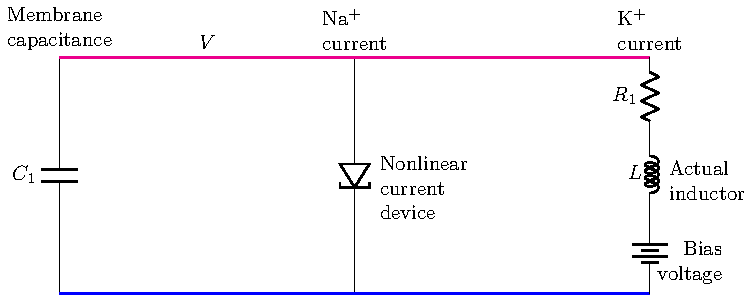
\includegraphics[width=0.18\pagewidth]{./Figures/Nagumo/Nagumo.pdf}
    \end{tikzfigure}
    \begin{tikzfigure}[Keener circuit layout]
      % \centering
      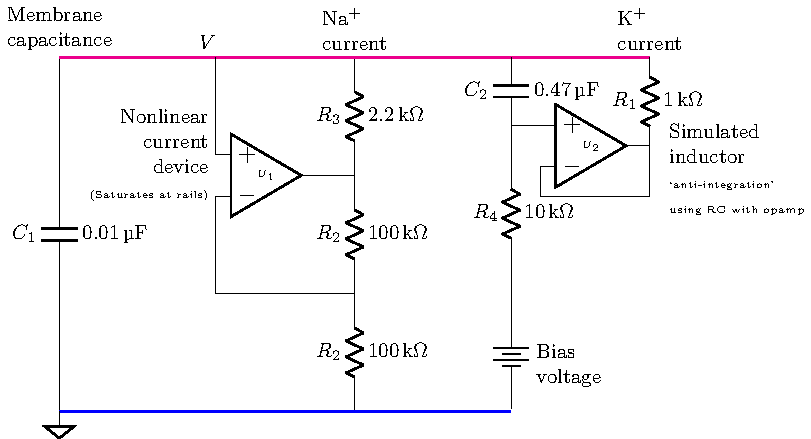
\includegraphics[width=0.19\pagewidth]{./Figures/NeuronUnit/NeuronUnit.pdf}
    \end{tikzfigure}
  \end{minipage}
  \begin{minipage}[b]{0.1\pagewidth}
    \begin{tikzfigure}[Nullclines]
      \centering
      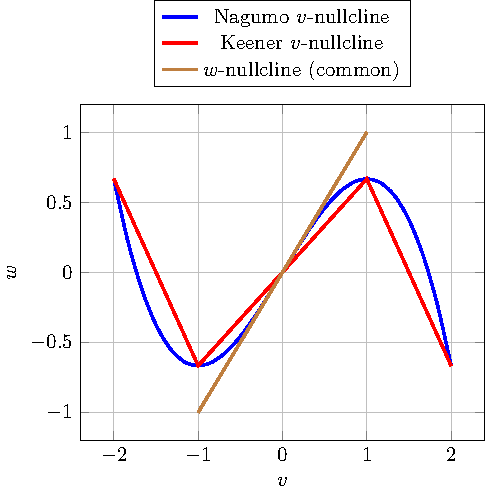
\includegraphics[width = 0.1\pagewidth]{./Figures/Nullclines/Nullclines.pdf}
    \end{tikzfigure}
  \end{minipage}

  This represents a single neuron.

  We have implemented a time-delay unidirectional diffusion using an R-C circuit (to simulate diffusion of neurotransmitter across a membrane), as well as negative unidirectional diffusion coupling using an inverting amplifier:

  \begin{minipage}[b]{0.15\pagewidth}
    \begin{tikzfigure}[Time-delay diffusion]
      \centering
      \includegraphics{./Figures/RCCoupler/RCCoupler.pdf}
    \end{tikzfigure}
  \end{minipage}
  \begin{minipage}[b]{0.15\pagewidth}
    \begin{tikzfigure}[Negative diffusion]
      \centering
      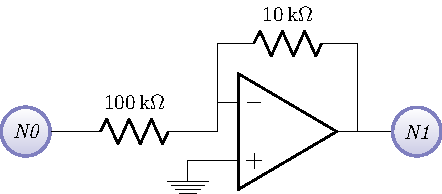
\includegraphics{./Figures/NegativeCoupling/NegativeCoupling.pdf}
    \end{tikzfigure}
  \end{minipage}



  }

  \block{Selected References}{
  \nocite{*}
  \singlespacing
  \normalsize
  \printbibliography[heading = none]
  }

  % \begin{array}{l}{d x_{0} / d t=x_{0}-x_{0}^{3} / 3-y_{0}+J} \\ {d y_{0} / d t=\varepsilon\left(x_{0}-\gamma y_{0}+\beta\right)} \\ {d x_{1} / d t=x_{1}-x_{1}^{3} / 3-y_{1}+J+D\left(x_{0}-x_{1}\right)} \\ {d y_{1} / d t=\varepsilon\left(x_{1}-\gamma y_{1}+\beta\right)}\end{array}

  % \block{Response}{
  %
  % This was the response of the circuit:
  % \begin{tikzfigure}[Two way diffusive coupling in circuit]
  %
  %   \centering
  %
  % \end{tikzfigure}
  %
  % and more will be forthcoming!
  % }

\end{columns}
\end{document}
